% Options for packages loaded elsewhere
\PassOptionsToPackage{unicode}{hyperref}
\PassOptionsToPackage{hyphens}{url}
\PassOptionsToPackage{dvipsnames,svgnames,x11names}{xcolor}
%
\documentclass[
  letterpaper,
  DIV=11,
  numbers=noendperiod]{scrartcl}

\usepackage{amsmath,amssymb}
\usepackage{iftex}
\ifPDFTeX
  \usepackage[T1]{fontenc}
  \usepackage[utf8]{inputenc}
  \usepackage{textcomp} % provide euro and other symbols
\else % if luatex or xetex
  \usepackage{unicode-math}
  \defaultfontfeatures{Scale=MatchLowercase}
  \defaultfontfeatures[\rmfamily]{Ligatures=TeX,Scale=1}
\fi
\usepackage{lmodern}
\ifPDFTeX\else  
    % xetex/luatex font selection
\fi
% Use upquote if available, for straight quotes in verbatim environments
\IfFileExists{upquote.sty}{\usepackage{upquote}}{}
\IfFileExists{microtype.sty}{% use microtype if available
  \usepackage[]{microtype}
  \UseMicrotypeSet[protrusion]{basicmath} % disable protrusion for tt fonts
}{}
\makeatletter
\@ifundefined{KOMAClassName}{% if non-KOMA class
  \IfFileExists{parskip.sty}{%
    \usepackage{parskip}
  }{% else
    \setlength{\parindent}{0pt}
    \setlength{\parskip}{6pt plus 2pt minus 1pt}}
}{% if KOMA class
  \KOMAoptions{parskip=half}}
\makeatother
\usepackage{xcolor}
\setlength{\emergencystretch}{3em} % prevent overfull lines
\setcounter{secnumdepth}{-\maxdimen} % remove section numbering
% Make \paragraph and \subparagraph free-standing
\ifx\paragraph\undefined\else
  \let\oldparagraph\paragraph
  \renewcommand{\paragraph}[1]{\oldparagraph{#1}\mbox{}}
\fi
\ifx\subparagraph\undefined\else
  \let\oldsubparagraph\subparagraph
  \renewcommand{\subparagraph}[1]{\oldsubparagraph{#1}\mbox{}}
\fi

\usepackage{color}
\usepackage{fancyvrb}
\newcommand{\VerbBar}{|}
\newcommand{\VERB}{\Verb[commandchars=\\\{\}]}
\DefineVerbatimEnvironment{Highlighting}{Verbatim}{commandchars=\\\{\}}
% Add ',fontsize=\small' for more characters per line
\usepackage{framed}
\definecolor{shadecolor}{RGB}{241,243,245}
\newenvironment{Shaded}{\begin{snugshade}}{\end{snugshade}}
\newcommand{\AlertTok}[1]{\textcolor[rgb]{0.68,0.00,0.00}{#1}}
\newcommand{\AnnotationTok}[1]{\textcolor[rgb]{0.37,0.37,0.37}{#1}}
\newcommand{\AttributeTok}[1]{\textcolor[rgb]{0.40,0.45,0.13}{#1}}
\newcommand{\BaseNTok}[1]{\textcolor[rgb]{0.68,0.00,0.00}{#1}}
\newcommand{\BuiltInTok}[1]{\textcolor[rgb]{0.00,0.23,0.31}{#1}}
\newcommand{\CharTok}[1]{\textcolor[rgb]{0.13,0.47,0.30}{#1}}
\newcommand{\CommentTok}[1]{\textcolor[rgb]{0.37,0.37,0.37}{#1}}
\newcommand{\CommentVarTok}[1]{\textcolor[rgb]{0.37,0.37,0.37}{\textit{#1}}}
\newcommand{\ConstantTok}[1]{\textcolor[rgb]{0.56,0.35,0.01}{#1}}
\newcommand{\ControlFlowTok}[1]{\textcolor[rgb]{0.00,0.23,0.31}{#1}}
\newcommand{\DataTypeTok}[1]{\textcolor[rgb]{0.68,0.00,0.00}{#1}}
\newcommand{\DecValTok}[1]{\textcolor[rgb]{0.68,0.00,0.00}{#1}}
\newcommand{\DocumentationTok}[1]{\textcolor[rgb]{0.37,0.37,0.37}{\textit{#1}}}
\newcommand{\ErrorTok}[1]{\textcolor[rgb]{0.68,0.00,0.00}{#1}}
\newcommand{\ExtensionTok}[1]{\textcolor[rgb]{0.00,0.23,0.31}{#1}}
\newcommand{\FloatTok}[1]{\textcolor[rgb]{0.68,0.00,0.00}{#1}}
\newcommand{\FunctionTok}[1]{\textcolor[rgb]{0.28,0.35,0.67}{#1}}
\newcommand{\ImportTok}[1]{\textcolor[rgb]{0.00,0.46,0.62}{#1}}
\newcommand{\InformationTok}[1]{\textcolor[rgb]{0.37,0.37,0.37}{#1}}
\newcommand{\KeywordTok}[1]{\textcolor[rgb]{0.00,0.23,0.31}{#1}}
\newcommand{\NormalTok}[1]{\textcolor[rgb]{0.00,0.23,0.31}{#1}}
\newcommand{\OperatorTok}[1]{\textcolor[rgb]{0.37,0.37,0.37}{#1}}
\newcommand{\OtherTok}[1]{\textcolor[rgb]{0.00,0.23,0.31}{#1}}
\newcommand{\PreprocessorTok}[1]{\textcolor[rgb]{0.68,0.00,0.00}{#1}}
\newcommand{\RegionMarkerTok}[1]{\textcolor[rgb]{0.00,0.23,0.31}{#1}}
\newcommand{\SpecialCharTok}[1]{\textcolor[rgb]{0.37,0.37,0.37}{#1}}
\newcommand{\SpecialStringTok}[1]{\textcolor[rgb]{0.13,0.47,0.30}{#1}}
\newcommand{\StringTok}[1]{\textcolor[rgb]{0.13,0.47,0.30}{#1}}
\newcommand{\VariableTok}[1]{\textcolor[rgb]{0.07,0.07,0.07}{#1}}
\newcommand{\VerbatimStringTok}[1]{\textcolor[rgb]{0.13,0.47,0.30}{#1}}
\newcommand{\WarningTok}[1]{\textcolor[rgb]{0.37,0.37,0.37}{\textit{#1}}}

\providecommand{\tightlist}{%
  \setlength{\itemsep}{0pt}\setlength{\parskip}{0pt}}\usepackage{longtable,booktabs,array}
\usepackage{calc} % for calculating minipage widths
% Correct order of tables after \paragraph or \subparagraph
\usepackage{etoolbox}
\makeatletter
\patchcmd\longtable{\par}{\if@noskipsec\mbox{}\fi\par}{}{}
\makeatother
% Allow footnotes in longtable head/foot
\IfFileExists{footnotehyper.sty}{\usepackage{footnotehyper}}{\usepackage{footnote}}
\makesavenoteenv{longtable}
\usepackage{graphicx}
\makeatletter
\def\maxwidth{\ifdim\Gin@nat@width>\linewidth\linewidth\else\Gin@nat@width\fi}
\def\maxheight{\ifdim\Gin@nat@height>\textheight\textheight\else\Gin@nat@height\fi}
\makeatother
% Scale images if necessary, so that they will not overflow the page
% margins by default, and it is still possible to overwrite the defaults
% using explicit options in \includegraphics[width, height, ...]{}
\setkeys{Gin}{width=\maxwidth,height=\maxheight,keepaspectratio}
% Set default figure placement to htbp
\makeatletter
\def\fps@figure{htbp}
\makeatother

\KOMAoption{captions}{tableheading}
\makeatletter
\makeatother
\makeatletter
\makeatother
\makeatletter
\@ifpackageloaded{caption}{}{\usepackage{caption}}
\AtBeginDocument{%
\ifdefined\contentsname
  \renewcommand*\contentsname{Table of contents}
\else
  \newcommand\contentsname{Table of contents}
\fi
\ifdefined\listfigurename
  \renewcommand*\listfigurename{List of Figures}
\else
  \newcommand\listfigurename{List of Figures}
\fi
\ifdefined\listtablename
  \renewcommand*\listtablename{List of Tables}
\else
  \newcommand\listtablename{List of Tables}
\fi
\ifdefined\figurename
  \renewcommand*\figurename{Figure}
\else
  \newcommand\figurename{Figure}
\fi
\ifdefined\tablename
  \renewcommand*\tablename{Table}
\else
  \newcommand\tablename{Table}
\fi
}
\@ifpackageloaded{float}{}{\usepackage{float}}
\floatstyle{ruled}
\@ifundefined{c@chapter}{\newfloat{codelisting}{h}{lop}}{\newfloat{codelisting}{h}{lop}[chapter]}
\floatname{codelisting}{Listing}
\newcommand*\listoflistings{\listof{codelisting}{List of Listings}}
\makeatother
\makeatletter
\@ifpackageloaded{caption}{}{\usepackage{caption}}
\@ifpackageloaded{subcaption}{}{\usepackage{subcaption}}
\makeatother
\makeatletter
\@ifpackageloaded{tcolorbox}{}{\usepackage[skins,breakable]{tcolorbox}}
\makeatother
\makeatletter
\@ifundefined{shadecolor}{\definecolor{shadecolor}{rgb}{.97, .97, .97}}
\makeatother
\makeatletter
\makeatother
\makeatletter
\makeatother
\ifLuaTeX
  \usepackage{selnolig}  % disable illegal ligatures
\fi
\IfFileExists{bookmark.sty}{\usepackage{bookmark}}{\usepackage{hyperref}}
\IfFileExists{xurl.sty}{\usepackage{xurl}}{} % add URL line breaks if available
\urlstyle{same} % disable monospaced font for URLs
\hypersetup{
  pdftitle={TP 4 : L'impact des débats électoraux sur le soutien électoral des partis politiques lors des élections Québécoises de 2022},
  pdfauthor={Olivia Saffioti},
  colorlinks=true,
  linkcolor={blue},
  filecolor={Maroon},
  citecolor={Blue},
  urlcolor={Blue},
  pdfcreator={LaTeX via pandoc}}

\title{TP 4 : L'impact des débats électoraux sur le soutien électoral
des partis politiques lors des élections Québécoises de 2022}
\author{Olivia Saffioti}
\date{}

\begin{document}
\maketitle
\ifdefined\Shaded\renewenvironment{Shaded}{\begin{tcolorbox}[enhanced, boxrule=0pt, sharp corners, frame hidden, breakable, interior hidden, borderline west={3pt}{0pt}{shadecolor}]}{\end{tcolorbox}}\fi

« There's more television being watched now (2015) than ever before
\ldots{} For the most part, voters tend to be 35 and older. These are
the people who statistically vote the most. So, that's why you still see
TV as your biggest megaphone », a exprimé Evan Tracey (vice president à
National Media Inc), dans un article sur la relation entre la télévision
et les élections (Shepard 2015). La télévision est devenue un outil de
communication politique important, car en tant que média de masse, ce
dernier touche un grand nombre d'individus. Les politiciens, en
particulier, utilisent souvent la télévision dans le cadre de leurs
campagnes électorales. En effet, « l'image des leaders, le marketing et
la communication visuelle des activités politiques » sont des
préoccupations importantes pour les organisations partisanes (Giasson
2006). Or, à travers la visibilité que la télévision lui octroie, un
chef de parti peut élargir la portée de sa campagne de communication à
un plus grand nombre d'électeurs. Il peut donc mobiliser davantage de
votes en les convaincant de ses « positions partisanes » et de son «
leadership » (Giasson 2006). En revanche, la littérature scientifique
reste mitigée sur les effets des débats électoraux sur le soutien
électoral. En effet, des recherches antérieures portant sur les
élections en Amérique Latine ont montré que les débats électoraux ne
faisaient que renforcer les préférences politiques prééxistantes des
électeurs (Cantu et Carreras 2023). D'autres recherches se centrant sur
les élections Allemandes ont montré que les débats électoraux
impactaient l'évaluation de l'image des candidats (Lindemann et Stoetzer
2021). Cependant, l'évaluation du programme et des promesses des partis
politiques ne changeait pas (\emph{Ibid} 2021). En revanche, les effets
des débats électoraux sur l'image des candidats seraient éphémères, et
n'impacteraient pas le soutien électoral des partis sur le long terme
(\emph{Ibid} 2021). À l'inverse, d'autres études se centrant sur les
États-Unis ont mis en exergue que les débats électoraux impactaient
l'évaluation des candidats et le choix de vote des citoyens (Schrott
1990; Shaw 1999). En revanche, nous n'avons pas trouvé de recherches
s'étant centrées sur le cas Québécois. Ainsi, il nous apparaissait
pertinent d'étudier le cas des élections Québécoises de 2022 afin de
vérifier si les débats électoraux ont impacté la popularité des partis
politiques dans les sondages. Nous avons choisi d'étudier les élections
Québecoises de 2022 car les sondages d'opinion qui ont été menés durant
les campagnes électorales de 2022 sont faciles d'accès. En effet, nous
avons trouvé un tableau regroupant les données des sondages de 2022 sur
Wikipédia. Or, Wikipédia demeure une plateforme sur laquelle les
contenus sont en libre-accès. Ce tableau constitue une base de données
pertinente et nous l'avons utilisé dans le cadre de notre recherche.
Nous avons choisi cette base de données pour plusieurs raisons. Tout
d'abord, elle indique à quelles dates des débats des chefs ont eu lieu
(la date du débat des chefs ayant eu lieu sur la chaîne TVA, et celle du
débat des chefs ayant eu lieu sur la chaîne de Radio-Canada). En outre,
il s'agit d'une base de données regroupant plusieurs sondages. Elle
spécifie également les sondeurs et les sources des sondages. Ainsi, la
base de données semble fiable en raison de sa transparence. Elle est
également complète en regroupant les sondages ayant été menés du 28 août
au 03 octobre 2022. Afin de mener notre recherche, nous allons faire du
web-scraping. Cela nous permettra d'importer la base de données de
Wikipédia sur R. Puis, nous allons nettoyer la base de données et nous
réaliserons un graphique. Puis, nous analyserons les résultats que nous
aurons obtenu.

\hypertarget{muxe9thode-et-donnuxe9es}{%
\subsection{Méthode et données}\label{muxe9thode-et-donnuxe9es}}

Afin de mener notre étude, nous avons récupéré des données de sondages
d'opinion issues de Wikipédia. Pour ce faire, nous avons fait du
``web-scraping''. Nous avons obtenu nos données en indiquant au logiciel
R le lien de la page Wikipédia et le tableau de cette page que nous
voulions scraper. Pour ce faire, nous avons utilisé les fonctions
read\_html(), html\_element(), pluck() et html\_table(). Le tableau que
nous souhaitions récupérer a ainsi été importé sur R. Il s'agissait du
tableau regroupant les données des sondages d'opinion menés lors des
élections québécoises de 2022. Ce tableau contenait plusieurs variables
: une variable intitulée ``dernier jour du sondage'' (relatant les dates
auxquels les différents sondages ont pris fin), une variable nommée
``source'' (indiquant le lien vers la source où se trouve les données
des sondages), une variable intitulée ``ME'' (spécifiant l'écart moyen
en pourcentage, soit à quel point les résultats sont précis et proches
de la valeur réelle de la population), une variable nommée
``Échantillon'' (spécifiant la taille des échantillons des sondages),
une variable intitulée ``Sondeur'' (qui spécifie quels sondeurs sont à
l'origine des différents sondages), et des variables représentant le
soutien électoral des partis politiques par jour (les résultats des
sondages). Ces variables se nomment ``CAQ'' (pour le parti Coalition
Avenir Québec), ``PLQ'' (pour le Parti Libéral du Québec''), ``PQ''
(pour le Parti Québécois), ``QS'' (pour le parti Québec Solidaire),
``PCQ'' (pour le Parti Conservateur du Québec) et ``Autres (pour les
autres partis politiques).

Nous avons nettoyé la base de données que nous avons importé sur R. Nous
avons commencé par retirer les lignes du tableau qui nous étaient
inutiles. En effet, dans certaines lignes du tableau se trouvaient des
informations textuelles. Par exemple, certaines indiquaient que des
débats des chefs avaient eu lieu le 15 et le 22 septembre 2022. Or,
garder ces lignes aurait complexifié la manipulation des données. En
effet, ces informations textuelles auraient été comprises comme des
données. C'est pourquoi, nous avons supprimé les lignes 1, 17, 29 et 50
de notre tableau grâce au code ``data{[}-c(1, 17, 29, 50), {]}''. En
outre, nous avons enlevé les colonnes de la base de données qui
n'étaient pas utiles pour notre recherche. Par exemple, la colonne 13
n'était pas nommée et affichait uniquement des valeurs ``NA''. Afin de
supprimer la colonne 13, nous avons utilisé le code ``data {[}, -13{]}''
. De plus, nous avions besoin de garder uniquement la colonne/variable
``date'' et les colonnes/variables représentants les partis politiques.
Afin de conserver uniquement les variables qui étaient pertinentes à
notre recherche, nous avons mobilisé le code ``data {[} , c(''date'',
``CAQ'', ``PLQ'', ``PQ'', ``QS'', ``PCQ'', ``Autres''){]}. Nous avons
également renommé la variable ``Dernier jour du sondage''. Nous l'avons
renommée ``date'' afin de rendre la base de données plus claire et plus
facile à interpréter. En outre, nous avons remplacé les tirets (``-'')
présents dans la colonne ``Autres''. Ces tirets représentaient les
valeurs manquantes. Afin de pouvoir manipuler les données de la variable
``Autres'' plus facilement, nous avons remplacé ces tirets par
l'abréviation ``NA'' qui signifie ``Not Available''. Ensuite, nous avons
changé le format des dates spécifiées dans la colonne ``date''. Nous les
avons converties en format day/month/year (dmy). Pour ce faire, nous
avons utilisé le code ``Sys.setlocale(''LC\_TIME'', ``fr\_FR'')'' afin
que le logiciel interprète les dates comme des dates françaises et que
nous puissions les formater. Afin de les formater, nous avons mobilisé
la fonction mutate(). Ensuite, nous avons réordonné les dates en ordre
chronologique. Pour ce faire, nous avons converti toutes nos variables
en format numérique grâce à la fonction as.numeric(). Puis, nous avons
converti les dates en format ``Date'' grâce à la fonction as.Date(), et
créé trois nouvelles colonnes relatant les jours, les mois et les
années. Ces colonnes nous ont permis par la suite de réorganiser les
dates chronologiquement. Pour créer ces colonnes, nous avons mobilisé
les fonctions mutate(), lubridate::year(), lubridate::month(), et
lubridate::day(). Puis, nous avons utilisé les fonctions group\_by(),
summarize(), et arrange(). Ces fonctions nous ont permis de réorganiser
les données de la variable ``date'' de manière chronologique, de
calculer les moyennes des résultats des sondages qui ont été menés le
même jour, et d'inclure ces moyennes dans nos données. Grâce à ces
moyennes, les données des variables ``CAQ'', ``PLQ'', ``PQ'', ``QS'',
``PCQ'' et ``Autres'' ont pu être simplifiées. Ainsi, nous pouvions les
analyser, les interpréter et les manipuler plus facilement en vue de
réaliser un graphique clair et lisible. Finalement, notre base de
données finale comprenait les variables suivantes : ``date'' (les dates
des sondages), ``year''(l'année des sondages), ``month'' (les mois
durant lequels les sondages ont été menés), ``day'' (les jours durant
lequels les sondages ont été menés), ``support\_moyen\_CAQ'' (le support
électoral moyen de la Coalition Avenir Québec à chaque date),
``support\_moyen\_PLQ'' (le support électoral moyen du Parti Libéral du
Québec à chaque date), ``support\_moyen\_PQ''(le support électoral moyen
du Parti Québécois à chaque date), ``support\_moyen\_QS'' (le support
électoral moyen de Québec Solidaire à chaque date),
support\_moyen\_PCQ'' (le support électoral moyen du Parti Conservateur
du Québec à chaque date), ``support\_moyen\_Autres'' (le support
électoral moyen des autres partis politiques à chaque date). Notre base
de données nettoyée est disponible en annexe, tout comme les codes que
nous avons mobilisé afin d'importer et de nettoyer notre de base de
données.

Enfin, nous avons réalisé un graphique à partir de notre base de données
nettoyée. Les codes utilisées afin de générer le graphique sont
eux-aussi placés en annexe.

\hypertarget{ruxe9sultats}{%
\subsection{Résultats}\label{ruxe9sultats}}

\includegraphics{/Users/oliviasaffioti/Desktop/graph.png}

Au sein du graphique ci-dessus, l'annotation ``Soutien après débat 1''
fait référence au soutien électoral suite au débat des chefs du 15
septembre 2022 organisé sur la chaîne TVA. L'annotation ``Soutien après
débat 2'', quant à elle, représente le soutien électoral suite au débat
des chefs ayant eu lieu le 22 septembre 2022 sur la chaîne Radio-Canada.

Les résultats que nous avons avons obtenu montrent que le soutien
électoral des partis politiques a varié suite aux débats des chefs. En
effet, le soutien électoral de la CAQ a baissé dans les sondages suite
au premier débat ayant lieu sur la chaîne TVA. En revanche, son soutien
électoral a augmenté suite au deuxième débat des chefs ayant eu lieu sur
la chaîne de Radio-Canada. La CAQ a fini par augmenté en popularité dans
les sondages par rapport au début de sa campagne ( par rapport au 28
août). Concernant le PQ, ce dernier a gagné en soutien électoral suite
aux débats de la chaîne TVA et de Radio-Canada. Le parti a gagné en
popularité par rapport au 28 août. En outre, le QS a gagné en popularité
suite au débat des chefs de la chaîne TVA, mais cette popularité a
baissé suite au débat des chefs de Radio-Canada. Dans l'ensemble, le QS
a augmenté légérément en popularité suite aux débats électoraux. De
plus, le PLQ a baissé en popularité dans les sondages suite au débat de
la chaîne TVA, et a légérement gagné en popularité suite au débat de
Radio-Canada. En revanche, sa popularité avait un niveau plus bas le 3
octobre par rapport au 28 août. De surcroît, la popularité du PCQ a
plutôt stagné suite au débat des chefs de la chaîne TVA, et a baissé
après que le débat de Radio-Canada ait eu lieu. Sa popularité était plus
basse lors du 03 octobre qu'elle ne l'était lors du 28 août. Finalement,
concernant les autres partis, leur popularité a baissé suite au deux
débats des chefs. Leur popularité était donc moins importante le 03
octobre qu'elle ne l'était le 28 août.

Donc, la popularité des partis politiques dans les sondages a augmenté
ou baissé suite aux deux débats des chefs qui ont lieu en 2022. Par
conséquent, les débats électoraux semblent avoir impacté l'évaluation
des candidats et des partis politiques par l'opinion publique. Ainsi,
les débats électoraux auraient impacté la popularité et le soutien
électoral des partis politiques selon les sondages d'opinion. Les bases
électorales des différents partis auraient pu être fracturées grâce au
débats des chefs, ce qui expliquerait que la popularité de certains
partis ait augmenté et que pour d'autres, leur soutien ait baissé. Mais
d'autres facteurs que les débats auraient pu permettre de fracturer
l'électorat. Par exemple d'autres éléments contextuels (économiques,
etc.) que nous n'avons pas pris en compte ou encore d'autres éléments
liés aux campagnes électorales des partis (scandales, polémiques,
stratégies de campagne comme les campagnes publicitaires, etc.) auraient
pu impacter le soutien électoral des partis politiques dans les
sondages. Finalement, notre hypothèse semble avérée mais notre recherche
mériterait d'être davantage poussée afin de vérifier si d'autres
variables sont intervenues et ont influencé le support électoral.

\hypertarget{conclusion}{%
\subsection{Conclusion}\label{conclusion}}

Pour conclure, nous avons mené du web-scraping afin d'importer une base
de données de Wikipédia sur R. Cette base de données regroupait les
résultats de différents sondages qui ont été menés entre le 28 août et
le 03 octobre, durant les élections Québécoises de 2022. Avec cette base
de données, nous avons étudié l'impact des débats électoraux sur le
soutien électoral des partis politiques. Nos résultats suggèrent que les
débats électoraux auraient eu un effet sur la popularité des partis
politiques dans les sondages, lors des élections de 2022. En revanche,
d'autres variables pourraient impacter la relation entre nos deux
variables. Par conséquent, notre étude contient des limites et
mériterait d'être menée à nouveau en incluant d'autres variables
explicatives. En outre, la méthode que nous avons mobilisé contient des
limites éthiques. En effet, bien que la base de données scrapée était en
libre accès sur Wikipédia, la question des droits d'auteur se pose.
Cette base de données avait été produite avec les résultats de plusieurs
sondages. Cependant, nous n'avons pas obtenu directement l'autorisation
des sondeurs pour utiliser et manipuler leurs données. Or, la
confidentialité des données pourrait être baffouée dans cette mesure
(Alexander 2023). En effet, même si les sondeurs avaient rendues
publiques leurs données dans un certain contexte, nous avons modifié ce
contexte en récupérant leurs données sur Wikipédia (Alexander 2023).
Cela met l'emphase sur des préoccupations éthiques importantes. Notre
méthode pousse à remettre en question les aspects légaux et éthiques de
la collecte et de l'utilisation de données issues de sources publiques.

\hypertarget{bibliographie}{%
\subsection{Bibliographie}\label{bibliographie}}

Alexander, Rohan. 2023. Telling Stories with Data: With Applications in
R. Chapman; Hall/CRC.
\url{https://tellingstorieswithdata.com/07-gather.html}

Cantú F., Carreras, M. 2023. ``Presidential Debates and Electoral
Preferences in Weakly Institutionalised Democracies: Evidence From 32
Latin American Elections''. \emph{Journal of Politics in Latin America}
15(3) : 239-261. \url{https://doi.org/10.1177/1866802X231213668}

Giasson, Thierry. 2006. « Les politiciens maîtrisent-ils leur image ? ».
\emph{Revue Communication} 25: 46-83.
\url{https://journals.openedition.org/communication/1633}

Lindemann Korinna , Stoetzer, Lukas F. 2021. ``The effect of televised
candidate debates on the support for political parties''.
\emph{Electoral Studies} 69 : 1-27.
\url{https://www.sciencedirect.com/science/article/pii/S0261379420301220}

Schrott PR.1990. ``Electoral consequences of ``winning'' televised
campaign debates''. \emph{Public Opinion Quarterly} 54(4): 567--585.
\url{https://academic.oup.com/poq/article/54/4/567/1909955}

Shaw DR. 1999. ``A study of presidential campaign event effects from
1952 to 1992''. \emph{The Journal of Politics} 61(2): 387--422.
\url{https://www.journals.uchicago.edu/doi/abs/10.2307/2647509}

Shepard, Steven. 2015. « The television election ». \emph{Politico,} 27
juillet, 2015.
\url{https://www.politico.com/story/2015/07/decline-of-tv-ads-not-in-2016-120611}

\hypertarget{annexe}{%
\subsection{Annexe}\label{annexe}}

\begin{Shaded}
\begin{Highlighting}[]
\CommentTok{\# Libraries}

\FunctionTok{library}\NormalTok{(tidyverse)}
\end{Highlighting}
\end{Shaded}

\begin{verbatim}
-- Attaching core tidyverse packages ------------------------ tidyverse 2.0.0 --
v dplyr     1.1.4     v readr     2.1.5
v forcats   1.0.0     v stringr   1.5.1
v ggplot2   3.4.4     v tibble    3.2.1
v lubridate 1.9.3     v tidyr     1.3.0
v purrr     1.0.2     
-- Conflicts ------------------------------------------ tidyverse_conflicts() --
x dplyr::filter() masks stats::filter()
x dplyr::lag()    masks stats::lag()
i Use the conflicted package (<http://conflicted.r-lib.org/>) to force all conflicts to become errors
\end{verbatim}

\begin{Shaded}
\begin{Highlighting}[]
\FunctionTok{library}\NormalTok{(lubridate)}
\FunctionTok{library}\NormalTok{(rvest)}
\end{Highlighting}
\end{Shaded}

\begin{verbatim}

Attaching package: 'rvest'

The following object is masked from 'package:readr':

    guess_encoding
\end{verbatim}

\begin{Shaded}
\begin{Highlighting}[]
\FunctionTok{library}\NormalTok{(scales)}
\end{Highlighting}
\end{Shaded}

\begin{verbatim}

Attaching package: 'scales'

The following object is masked from 'package:purrr':

    discard

The following object is masked from 'package:readr':

    col_factor
\end{verbatim}

\begin{Shaded}
\begin{Highlighting}[]
\CommentTok{\# Importer les données}

\NormalTok{Polls\_data }\OtherTok{\textless{}{-}} \FunctionTok{read\_html}\NormalTok{(}\StringTok{"https://fr.wikipedia.org/wiki/Liste\_de\_sondages\_sur\_les\_\%C3\%A9lections\_g\%C3\%A9n\%C3\%A9rales\_qu\%C3\%A9b\%C3\%A9coises\_de\_2022"}\NormalTok{)}

\NormalTok{Polls\_data }\OtherTok{\textless{}{-}}\NormalTok{ Polls\_data }\SpecialCharTok{\%\textgreater{}\%} \FunctionTok{html\_elements}\NormalTok{(}\StringTok{"table"}\NormalTok{) }\SpecialCharTok{\%\textgreater{}\%} \FunctionTok{pluck}\NormalTok{(}\DecValTok{2}\NormalTok{) }\SpecialCharTok{\%\textgreater{}\%} \FunctionTok{html\_table}\NormalTok{(}\AttributeTok{fill =}\NormalTok{ T)}

\CommentTok{\# Nettoyer les données}

\NormalTok{Polls\_data\_2 }\OtherTok{\textless{}{-}}\NormalTok{ Polls\_data[}\SpecialCharTok{{-}}\FunctionTok{c}\NormalTok{(}\DecValTok{1}\NormalTok{, }\DecValTok{17}\NormalTok{, }\DecValTok{29}\NormalTok{, }\DecValTok{50}\NormalTok{), ]}

\NormalTok{Polls\_data\_new }\OtherTok{\textless{}{-}}\NormalTok{ Polls\_data\_2[, }\SpecialCharTok{{-}}\DecValTok{13}\NormalTok{]}

\NormalTok{Polls\_data\_new }\OtherTok{\textless{}{-}}\NormalTok{ Polls\_data\_new }\SpecialCharTok{\%\textgreater{}\%} \FunctionTok{rename}\NormalTok{(}\AttributeTok{date =} \StringTok{"Dernier jourdu sondage"}\NormalTok{)}

\NormalTok{Polls\_data\_new }\OtherTok{\textless{}{-}}\NormalTok{ Polls\_data\_new [ , }\FunctionTok{c}\NormalTok{(}\StringTok{"date"}\NormalTok{, }\StringTok{"CAQ"}\NormalTok{, }\StringTok{"PLQ"}\NormalTok{, }\StringTok{"PQ"}\NormalTok{, }\StringTok{"QS"}\NormalTok{, }\StringTok{"PCQ"}\NormalTok{, }\StringTok{"Autres"}\NormalTok{)]}

\NormalTok{Polls\_data\_new }\OtherTok{\textless{}{-}}\NormalTok{ Polls\_data\_new }\SpecialCharTok{\%\textgreater{}\%} \FunctionTok{mutate}\NormalTok{(}\AttributeTok{Autres =} \FunctionTok{na\_if}\NormalTok{(Autres, }\StringTok{"{-}"}\NormalTok{))}

\FunctionTok{Sys.setlocale}\NormalTok{(}\StringTok{"LC\_TIME"}\NormalTok{, }\StringTok{"fr\_FR"}\NormalTok{)}
\end{Highlighting}
\end{Shaded}

\begin{verbatim}
[1] "fr_FR"
\end{verbatim}

\begin{Shaded}
\begin{Highlighting}[]
\NormalTok{Polls\_data\_nouveau }\OtherTok{\textless{}{-}}\NormalTok{ Polls\_data\_new }\SpecialCharTok{\%\textgreater{}\%} \FunctionTok{mutate}\NormalTok{(}\AttributeTok{date =} \FunctionTok{dmy}\NormalTok{(date))}

\NormalTok{Polls\_data\_nouveau }\OtherTok{\textless{}{-}}\NormalTok{ Polls\_data\_nouveau }\SpecialCharTok{\%\textgreater{}\%} \FunctionTok{mutate}\NormalTok{(}\AttributeTok{date =} \FunctionTok{format}\NormalTok{(date, }\StringTok{"\%d{-}\%m{-}\%Y"}\NormalTok{))}

\NormalTok{Polls\_data\_nouveau}\SpecialCharTok{$}\NormalTok{CAQ }\OtherTok{\textless{}{-}} \FunctionTok{as.numeric}\NormalTok{(Polls\_data\_nouveau}\SpecialCharTok{$}\NormalTok{CAQ)}

\NormalTok{Polls\_data\_nouveau}\SpecialCharTok{$}\NormalTok{PLQ}\OtherTok{\textless{}{-}} \FunctionTok{as.numeric}\NormalTok{(Polls\_data\_nouveau}\SpecialCharTok{$}\NormalTok{PLQ)}

\NormalTok{Polls\_data\_nouveau}\SpecialCharTok{$}\NormalTok{PQ }\OtherTok{\textless{}{-}} \FunctionTok{as.numeric}\NormalTok{(Polls\_data\_nouveau}\SpecialCharTok{$}\NormalTok{PQ)}

\NormalTok{Polls\_data\_nouveau}\SpecialCharTok{$}\NormalTok{QS }\OtherTok{\textless{}{-}} \FunctionTok{as.numeric}\NormalTok{(Polls\_data\_nouveau}\SpecialCharTok{$}\NormalTok{QS)}

\NormalTok{Polls\_data\_nouveau}\SpecialCharTok{$}\NormalTok{PCQ}\OtherTok{\textless{}{-}} \FunctionTok{as.numeric}\NormalTok{(Polls\_data\_nouveau}\SpecialCharTok{$}\NormalTok{PCQ)}

\NormalTok{Polls\_data\_nouveau}\SpecialCharTok{$}\NormalTok{Autres }\OtherTok{\textless{}{-}} \FunctionTok{as.numeric}\NormalTok{(Polls\_data\_nouveau}\SpecialCharTok{$}\NormalTok{Autres)}

\NormalTok{Polls\_data\_nouveau }\OtherTok{\textless{}{-}}\NormalTok{ Polls\_data\_nouveau }\SpecialCharTok{\%\textgreater{}\%} \FunctionTok{mutate}\NormalTok{(}\AttributeTok{date =} \FunctionTok{as.Date}\NormalTok{(date, }\AttributeTok{format =} \StringTok{"\%d{-}\%m{-}\%Y"}\NormalTok{), }\AttributeTok{year =}\NormalTok{ lubridate}\SpecialCharTok{::}\FunctionTok{year}\NormalTok{(date), }\AttributeTok{month =}\NormalTok{ lubridate}\SpecialCharTok{::}\FunctionTok{month}\NormalTok{(date), }\AttributeTok{day =}\NormalTok{ lubridate}\SpecialCharTok{::}\FunctionTok{day}\NormalTok{(date))}

\NormalTok{Polls\_data\_final }\OtherTok{\textless{}{-}}\NormalTok{ Polls\_data\_nouveau }\SpecialCharTok{\%\textgreater{}\%} \FunctionTok{group\_by}\NormalTok{(date, year, month, day) }\SpecialCharTok{\%\textgreater{}\%} \FunctionTok{summarize}\NormalTok{(}\AttributeTok{support\_moyen\_CAQ =} \FunctionTok{mean}\NormalTok{(CAQ, }\AttributeTok{na.rm =} \ConstantTok{TRUE}\NormalTok{), }\AttributeTok{support\_moyen\_PLQ =} \FunctionTok{mean}\NormalTok{(PLQ, }\AttributeTok{na.rm =} \ConstantTok{TRUE}\NormalTok{), }\AttributeTok{support\_moyen\_PQ =} \FunctionTok{mean}\NormalTok{(PQ, }\AttributeTok{na.rm =} \ConstantTok{TRUE}\NormalTok{), }\AttributeTok{support\_moyen\_QS =} \FunctionTok{mean}\NormalTok{(QS, }\AttributeTok{na.rm =} \ConstantTok{TRUE}\NormalTok{), }\AttributeTok{support\_moyen\_PCQ =} \FunctionTok{mean}\NormalTok{(PCQ, }\AttributeTok{na.rm =} \ConstantTok{TRUE}\NormalTok{), }\AttributeTok{support\_moyen\_Autres =} \FunctionTok{mean}\NormalTok{(Autres, }\AttributeTok{na.rm =} \ConstantTok{TRUE}\NormalTok{)) }\SpecialCharTok{\%\textgreater{}\%} \FunctionTok{arrange}\NormalTok{(year, month, day)}
\end{Highlighting}
\end{Shaded}

\begin{verbatim}
`summarise()` has grouped output by 'date', 'year', 'month'. You can override
using the `.groups` argument.
\end{verbatim}

\begin{Shaded}
\begin{Highlighting}[]
\FunctionTok{glimpse}\NormalTok{(Polls\_data\_final)}
\end{Highlighting}
\end{Shaded}

\begin{verbatim}
Rows: 36
Columns: 10
Groups: date, year, month [36]
$ date                 <date> 2022-08-28, 2022-08-29, 2022-08-30, 2022-08-31, ~
$ year                 <dbl> 2022, 2022, 2022, 2022, 2022, 2022, 2022, 2022, 2~
$ month                <dbl> 8, 8, 8, 8, 9, 9, 9, 9, 9, 9, 9, 9, 9, 9, 9, 9, 9~
$ day                  <int> 28, 29, 30, 31, 1, 2, 3, 4, 5, 6, 7, 8, 9, 10, 11~
$ support_moyen_CAQ    <dbl> 38.0, 40.0, 41.0, 39.0, 38.0, 37.0, 38.0, 39.0, 3~
$ support_moyen_PLQ    <dbl> 17.0, 19.0, 18.0, 20.0, 18.0, 18.0, 18.0, 18.0, 1~
$ support_moyen_PQ     <dbl> 7.0, 8.0, 7.0, 7.0, 8.0, 8.0, 9.0, 11.0, 11.0, 11~
$ support_moyen_QS     <dbl> 12, 12, 12, 13, 13, 13, 13, 12, 12, 11, 11, 11, 1~
$ support_moyen_PCQ    <dbl> 21.0, 18.0, 18.0, 17.0, 20.0, 20.0, 18.0, 18.0, 1~
$ support_moyen_Autres <dbl> 4.0, 4.0, 4.0, 5.0, 3.0, 4.0, 4.0, 4.0, 5.0, 5.0,~
\end{verbatim}

\begin{Shaded}
\begin{Highlighting}[]
\CommentTok{\# Faire le graphique}

\NormalTok{graph }\OtherTok{\textless{}{-}} \FunctionTok{ggplot}\NormalTok{(Polls\_data\_final, }\FunctionTok{aes}\NormalTok{(}\AttributeTok{x =}\NormalTok{ date)) }\SpecialCharTok{+} \FunctionTok{geom\_line}\NormalTok{(}\FunctionTok{aes}\NormalTok{(}\AttributeTok{y =}\NormalTok{ support\_moyen\_CAQ, }\AttributeTok{color =} \StringTok{"CAQ"}\NormalTok{)) }\SpecialCharTok{+} \FunctionTok{geom\_line}\NormalTok{(}\FunctionTok{aes}\NormalTok{(}\AttributeTok{y =}\NormalTok{ support\_moyen\_PLQ, }\AttributeTok{color =} \StringTok{"PLQ"}\NormalTok{)) }\SpecialCharTok{+} \FunctionTok{geom\_line}\NormalTok{(}\FunctionTok{aes}\NormalTok{(}\AttributeTok{y =}\NormalTok{ support\_moyen\_PQ, }\AttributeTok{color =} \StringTok{"PQ"}\NormalTok{)) }\SpecialCharTok{+} \FunctionTok{geom\_line}\NormalTok{(}\FunctionTok{aes}\NormalTok{(}\AttributeTok{y =}\NormalTok{ support\_moyen\_QS, }\AttributeTok{color =} \StringTok{"QS"}\NormalTok{)) }\SpecialCharTok{+} \FunctionTok{geom\_line}\NormalTok{(}\FunctionTok{aes}\NormalTok{(}\AttributeTok{y =}\NormalTok{ support\_moyen\_PCQ, }\AttributeTok{color =} \StringTok{"PCQ"}\NormalTok{)) }\SpecialCharTok{+} \FunctionTok{geom\_line}\NormalTok{(}\FunctionTok{aes}\NormalTok{(}\AttributeTok{y =}\NormalTok{ support\_moyen\_Autres, }\AttributeTok{color =} \StringTok{"Autres"}\NormalTok{)) }\SpecialCharTok{+} \FunctionTok{labs}\NormalTok{(}\AttributeTok{title =} \StringTok{"L\textquotesingle{}effet des débats des chefs sur l\textquotesingle{}évolution du soutien électoral par parti politique en 2022 "}\NormalTok{, }\AttributeTok{x =} \StringTok{"Dates"}\NormalTok{, }\AttributeTok{y =} \StringTok{"Soutien électoral moyen (en \%)"}\NormalTok{, }\AttributeTok{color =} \StringTok{"Partis politiques"}\NormalTok{) }\SpecialCharTok{+} \FunctionTok{theme\_minimal}\NormalTok{() }\SpecialCharTok{+} \FunctionTok{theme}\NormalTok{(}\AttributeTok{plot.title =} \FunctionTok{element\_text}\NormalTok{(}\AttributeTok{size =} \DecValTok{12}\NormalTok{), }\AttributeTok{axis.title.x =} \FunctionTok{element\_text}\NormalTok{ (}\AttributeTok{size =} \DecValTok{9}\NormalTok{), }\AttributeTok{axis.text.x =} \FunctionTok{element\_text}\NormalTok{(}\AttributeTok{angle =} \DecValTok{45}\NormalTok{,  }\AttributeTok{size =} \DecValTok{9}\NormalTok{), }\AttributeTok{axis.title.y =} \FunctionTok{element\_text}\NormalTok{(}\AttributeTok{size =} \DecValTok{9}\NormalTok{)) }\SpecialCharTok{+} \FunctionTok{scale\_color\_manual}\NormalTok{(}\AttributeTok{values =} \FunctionTok{c}\NormalTok{(}\StringTok{"CAQ"} \OtherTok{=} \StringTok{"orchid"}\NormalTok{, }\StringTok{"PLQ"} \OtherTok{=} \StringTok{"red"}\NormalTok{, }\StringTok{"PQ"} \OtherTok{=} \StringTok{"green"}\NormalTok{, }\StringTok{"QS"} \OtherTok{=} \StringTok{"orange"}\NormalTok{, }\StringTok{"PCQ"} \OtherTok{=} \StringTok{"blue"}\NormalTok{, }\StringTok{"Autres"} \OtherTok{=} \StringTok{"darkgray"}\NormalTok{)) }\SpecialCharTok{+} \FunctionTok{geom\_vline}\NormalTok{(}\AttributeTok{xintercept =} \FunctionTok{as.Date}\NormalTok{(}\FunctionTok{c}\NormalTok{(}\StringTok{"2022{-}09{-}15"}\NormalTok{, }\StringTok{"2022{-}09{-}22"}\NormalTok{)), }\AttributeTok{linetype =} \StringTok{"dashed"}\NormalTok{) }\SpecialCharTok{+} \FunctionTok{annotate}\NormalTok{(}\StringTok{"text"}\NormalTok{, }\AttributeTok{x =} \FunctionTok{as.Date}\NormalTok{(}\StringTok{"2022{-}09{-}15"}\NormalTok{), }\AttributeTok{y =} \ConstantTok{Inf}\NormalTok{, }\AttributeTok{label =} \StringTok{"Soutien après débat 1"}\NormalTok{, }\AttributeTok{fontface =} \StringTok{"bold"}\NormalTok{, }\AttributeTok{vjust =} \DecValTok{1}\NormalTok{, }\AttributeTok{hjust =} \SpecialCharTok{{-}}\FloatTok{0.02}\NormalTok{, }\AttributeTok{size =} \FloatTok{2.2}\NormalTok{) }\SpecialCharTok{+} \FunctionTok{annotate}\NormalTok{(}\StringTok{"text"}\NormalTok{, }\AttributeTok{x =} \FunctionTok{as.Date}\NormalTok{(}\StringTok{"2022{-}09{-}22"}\NormalTok{), }\AttributeTok{y =} \ConstantTok{Inf}\NormalTok{, }\AttributeTok{label =} \StringTok{"Soutien après débat 2"}\NormalTok{, }\AttributeTok{fontface =} \StringTok{"bold"}\NormalTok{, }\AttributeTok{vjust =} \DecValTok{1}\NormalTok{, }\AttributeTok{hjust =} \SpecialCharTok{{-}}\FloatTok{0.4}\NormalTok{, }\AttributeTok{size =} \FloatTok{2.2}\NormalTok{) }\SpecialCharTok{+} \FunctionTok{scale\_x\_date}\NormalTok{(}\AttributeTok{breaks =} \FunctionTok{as.Date}\NormalTok{(}\FunctionTok{c}\NormalTok{(}\StringTok{"2022{-}08{-}29"}\NormalTok{, }\StringTok{"2022{-}09{-}05"}\NormalTok{, }\StringTok{"2022{-}09{-}12"}\NormalTok{, }\StringTok{"2022{-}09{-}15"}\NormalTok{, }\StringTok{"2022{-}09{-}19"}\NormalTok{, }\StringTok{"2022{-}09{-}22"}\NormalTok{, }\StringTok{"2022{-}09{-}26"}\NormalTok{, }\StringTok{"2022{-}10{-}03"}\NormalTok{)), }\AttributeTok{labels =} \FunctionTok{date\_format}\NormalTok{(}\StringTok{"\%d \%b"}\NormalTok{))}

\NormalTok{graph}
\end{Highlighting}
\end{Shaded}

\begin{figure}[H]

{\centering 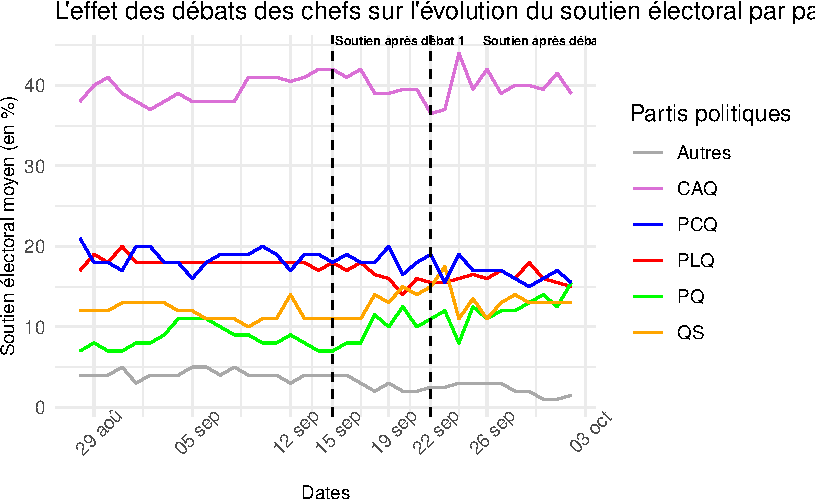
\includegraphics{TP4-FAS1001_files/figure-pdf/unnamed-chunk-1-1.pdf}

}

\end{figure}



\end{document}
